\graphicspath{ {3-FUNDAMENTOS/} }

\chapter{Fundamentação Teórica}
\label{sgbd}

Um ativo importante em qualquer organização é a informação. Segundo Kimball e Ross \cite{kimball2002dw} essa informação é mantida sob duas formas: sistemas de banco de dados operacionais e \textit{Data Warehouses}. Em sistemas operacionais geralmente os usuários lidam com o mesmo registro e realizam a mesma tarefa exaustivamente sob uma única informação, permanecendo no domínio das transações; enquanto que em um DW pode-se ver o progresso da organização utilizando dados armazenados continuamente, de forma otimizada para a recuperação de dados. Também, são formuladas perguntas com a finalidade de responder a alguma questão de negócio, como \textit{"quantos pedidos foram recebidos pelo fornecedor X no período de tempo Y?"}, ou \textit{"qual foi o impacto no número de vendas ao mudar o formato de envio de A para B?"}. Para responder questões dessa natureza não é viável lidar com dados de forma individual, mas sim recuperar um conjunto de dados a fim de formular uma resposta.

De acordo com Inmon \cite{inmon2005building}, DWs são base de todos os Sistemas de Suporte à Decisão (do inglês \textit{Decision Support Systems}, ou DSS). DSS são tecnologias utilizadas para decisões de negócio e solução de problemas, 
e incluem componentes que realizam gerenciamento de banco de dados e que 
permitem uma interação com o usuário de forma a simplificar consultas e geração de relatórios 
\cite{shim2002past}. DWs foram as primeiras ferramentas a surgirem como solução para o 
suporte à decisão de negócio, integrando dados de diferentes bancos de dados operacionais 
\cite{inmon2005building, kimball2002dw}.

De forma geral, um DW é um repositório de dados capaz de fornecer rapidamente 
informações consistentes e cruciais para a tomada de decisão de uma organização, 
de tal forma que essa informação possa ser acessada de maneira intuitiva e legível 
pelo usuário, a fim de combinar diferentes informações entre os dados armazenados 
\cite{kimball2002dw}. Deve também se adaptar a possíveis mudanças, sejam elas mudanças comerciais, mudanças nos dados ou na tecnologia. Inmon \cite{inmon2005building} define um DW como "uma coleção de dados não-volátil, ou seja, que não muda após inserida no \textit{warehouse}; orientado ao assunto principal da organização; integrado e variante no tempo para que seja mantido um histórico a fim de analisar situações passadas". Do ponto de vista estrutural, Wremble e Koncilia \cite{wrembel2007data} definem um DW como uma base de dados homogênea, local e centralizada.

Para analisar os dados de um DW além de implementá-lo é necessário que alguma aplicação leia seu conteúdo e apresente-o de forma gráfica e intuitiva ao analisador. Aplicações OLTP (\textit{On-Line Transactional Processing}) são utilizadas por bancos de dados operacionais e operam transações atômicas e isoladas de forma repetitiva, que correspondem ao dia-a-dia de uma organização \cite{chaudhuri1997overview}. DWs trabalham com suporte à decisão e são intensivos à consultas \textit{ad hoc} complexas, que acessam milhões de registros. Sendo assim, os dados históricos, a taxa de vazão de uma consulta e o tempo de resposta são mais importantes que pequenas transações.

À aplicação aceita por um DW dá-se o nome de OLAP, cujo objetivo, de acordo com Codd; Codd e Salley \cite{codd1998providing}, é identificar tendências, padrões de comportamento e anomalias, bem como relações em dados aparentemente não relacionados. Geralmente as consultas em uma aplicação analítica são longas, levam tempo para executar e estão interessadas 
em atributos específicos. Os resultados dessas análises servem de base para tomada de decisões de negócio. Ainda, o processo de inserção de dados em um ambiente OLAP é um pouco mais complexo que sistemas OLTP por seguir um processo fim-a-fim conhecido 
como ETL (extração, transformação e carga, do inglês \textit{extract, transformation, load}) \cite{vertabelo2017olap}. Portanto, DWs e aplicações OLAP são componentes chave para a construção de um ambiente de análise.

O processo ETL faz parte da arquitetura de um DW. Neste domínio existem diversos componentes que realizam funções específicas a fim de construir um ambiente de \textit{warehouse} desde a obtenção dos dados de fontes externas e sistemas operacionais de bancos de dados, até o acesso a esses dados por meio do DW por alguma consulta analítica definida sob uma aplicação OLAP. Para entender esta arquitetura fim-a-fim, ilustrada na Figura \ref{fig:dw_arq} adaptada de Kimball e Ross \cite{kimball2002dw}, é necessário compreender alguns componentes e conceitos que formam um DW \cite{kimball2002dw}:

\begin{itemize}
    \item \textbf{Sistemas de Fonte Operacional}: possuem detalhes sobre as transações do negócio, correspondendo a ambientes OLTP. Engloba os dados que irão estruturar as informações do DW, portanto, se encontram externos ao \textit{warehouse}. Podem ser tanto sistemas de banco de dados ou alguma outra fonte de dados, como um documento no formato XLS, CSV, TXT; e sistemas CRM.
    \item \textbf{\textit{Staging Area}}: compreende tanto uma área de armazenamento temporária quanto um conjunto de processos denominado ETL. De forma geral é uma área a qual os usuários não têm acesso, onde os dados são traduzidos para algo que possa ser enviado de maneira compatível ao \textit{warehouse} e não se trabalha diretamente sobre os dados transacionais. Quanto aos processos ETL, a fase de Extração (\textit{Extraction}) consiste na leitura da fonte de dados, transferindo o conteúdo necessário para a \textit{staging area}; após essa extração pode ser necessário realizar uma "limpeza" nos dados; unir dados de diferentes fontes; tratar duplicatas e atribuir chaves do \textit{warehouse}. A isto dá-se o nome de Transformação (\textit{Transformation}). A última fase, fase de Carga (\textit{Load}), é responsável por carregar, ou popular, os dados na área de estruturação de dados do DW.
    \item \textbf{Estruturação de Dados}: trata de como os dados serão organizados, armazenados e disponibilizados para consultas de usuários, relatórios e outras aplicações. No que tange à comunidade empresarial, a fase de apresentação de dados \textit{é} o DW em si, pois corresponde ao que pode ser acessado via ferramentas de acesso a dados. A etapa de estruturação é comumente definida como sendo um conjunto de \textit{data marts}. \textit{Data marts} são subconjuntos do total de informações de um DW, cada qual representando os dados de um determinado assunto, departamento, ou processo de negócio. Nesta fase é definida a modelagem conceitual do ambiente de análise do DW.
    \item \textbf{Ferramentas de Acesso aos Dados}: são formas de aplicar uma consulta, dentro de aplicações OLAP, aos dados organizados na fase de estruturação. Pode ser uma consulta \textit{ad hoc} ou algo mais complexo, como consultas aplicadas à mineração de dados.
    
\end{itemize}

\begin{figure*}[htpb]
	\centering
		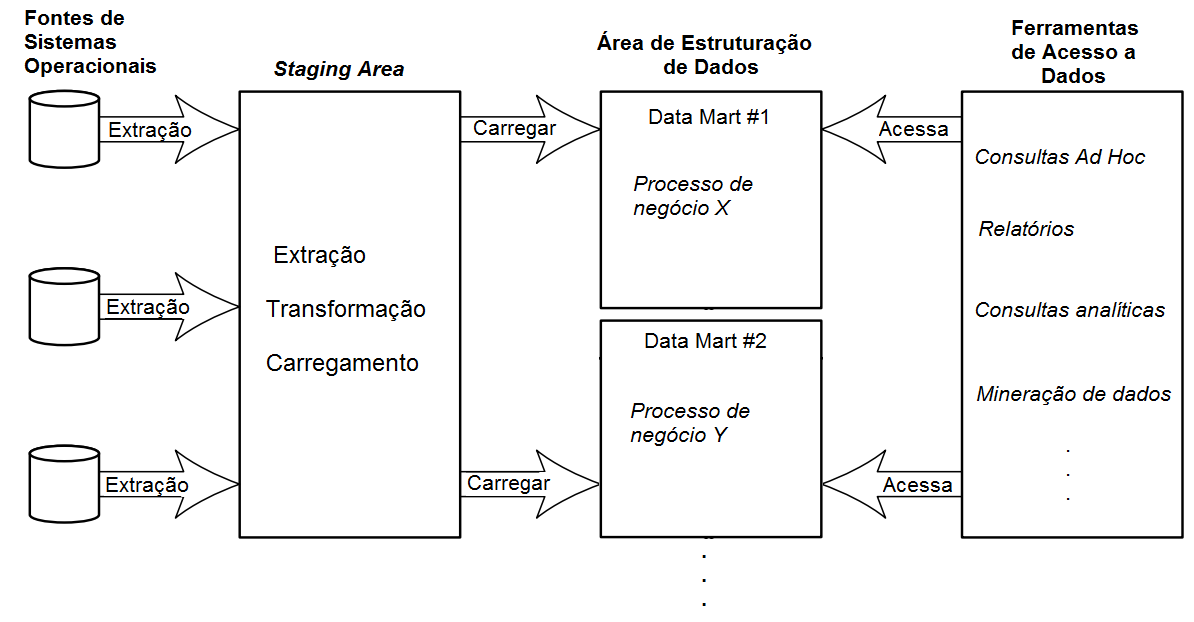
\includegraphics[width=\textwidth]{img/dw_arc}
    \caption{Arquitetura de um \textit{Data Warehouse}}
    % \floatfoot{Fonte: Kimball e Ross \cite{kimball2002dw}}
	\label{fig:dw_arq}
\end{figure*}

Existe uma discussão acerca da modelagem conceitual da área de apresentação de dados de um ambiente de análise nos DWs \cite{sen2005comparison}. Segundo Sen e Sinha \cite{sen2005comparison} as duas técnicas de modelagem mais utilizadas são a Entidade-Relacional (ER) e a Dimensional. A primeira segue o padrão de modelagem para ambientes OLTP, que traduz a modelagem ER para um esquema relacional em seguida normalizando-o geralmente até a Terceira Forma Normal (3NF) \cite{kimball2002dw}, normalmente utilizadas por banco de dados relacionais. O modelo Dimensional, ou multidimensional, por sua vez, evita atingir o mesmo nível de normalização da modelagem ER, e faz analogia a um cubo para representação de dados, uma vez que uma informação pode ser vista através de \textit{n} dimensões. 

O modelo dimensional é composto por tabelas denominadas Tabelas Fato e Tabelas Dimensão \cite{kimball2002dw}, e é conhecido comumente como modelo \textit{star join}, ou apenas \textit{star} \cite{sen2005comparison}, pelo seu formato lembrar o de uma estrela. A Tabela Fato é a principal tabela do modelo Dimensional, contemplando atributos responsáveis por determinar as regras e métricas de negócio, ou um fato. Em sua maioria são atributos numéricos, relacionados a quantidade, e aditivos, visto que uma consulta em um DW pode retornar até milhares de tuplas, tornando interessante o conhecimento de informações como o total de um atributo dada alguma questão de negócio. Atributos textuais não são definidos como um fato, na maioria das vezes descrevem algo e devem estar inseridos em Tabelas Dimensão pois há maior chance de estarem relacionados com os atributos dimensão. Outro ponto a se ater é a importância de se evitar incluir dados com zeros que não representam dados úteis, ou representando nada, pois a inclusão de dados sem significado sobrecarregariam o DW sem motivo.

As Tabelas Fato são auxiliadas pelas Tabelas Dimensão no que concerne à descrição textual das questões de negócio. É comum essas tabelas terem de 50 a 100 atributos, ou mais, pois a intenção das dimensões é descrever as regras de negócio. É nestas tabelas que são realizados os filtros de consulta. Por filtros entende-se agrupamentos, padrões e ordenações por exemplo. De forma a exemplificar, se fosse desejado buscar as vendas por nome de fornecedor em um determinado intervalo de data, os atributos "nome de fornecedor" e "data" deveriam estar armazenados em tabelas dimensão. Segundo Kimball \cite{kimball2002dw}, quanto mais bem descritos os atributos dimensão, melhor o DW é, tornando a qualidade do \textit{warehouse} dependente das entidades de dimensão.

Todas as Tabelas Fato tem duas ou mais chaves relacionando-as às Tabelas Dimensão, como mostra o exemplo da Figura \ref{fig:star_dim}, onde a tabela \textit{Vendas} corresponde à uma Tabela Fato e as demais à Tabelas Dimensão. Note que esta figura também faz referência a um modelo \textit{star}.

\begin{figure*}[htpb]
	\centering
		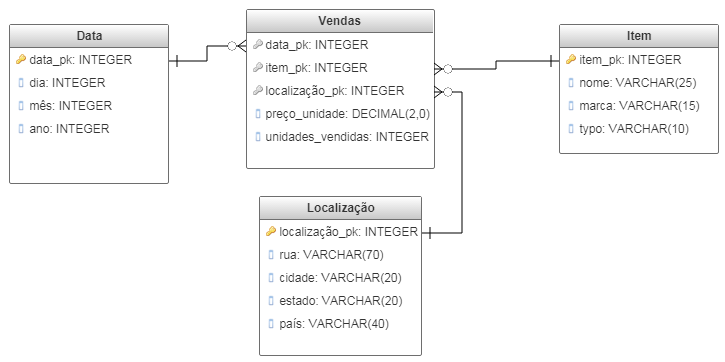
\includegraphics[width=13cm]{img/star_dim}
	\caption{Exemplo de esquema \textit{star} com tabelas Fato e Dimensão}
	\label{fig:star_dim}
\end{figure*}

Mesmo que a modelagem Dimensional não atinja a normalização 3NF, modelos \textit{star} podem ser trabalhados de forma a oferecer suporte à hierarquia de atributos às Tabelas Dimensão, permitindo que estas tenham Tabelas "Subdimensão". A esse refinamento se dá o nome de \textit{snowflake} \cite{navathe2011banco}. Embora tenham uma estrutura mais simplificada, segundo Levene e Loizou \cite{levene2003snowflake} a escolha do uso de esquemas \textit{snowflake} se dá por serem um esquema intuitivo, de fácil entendimento, passíveis à otimização de consultas, e de fácil extensão -- uma vez que pode-se adicionar atributos às tabelas sem interferir em programas já existentes. Uma possível adaptação de um modelo \textit{star} para \textit{snowflake} é como mostrado na Figura \ref{fig:snow}, no qual foi adaptado o modelo da Figura \ref{fig:star_dim}, adicionando a Tabela Subdimensão Cidade. 

\begin{figure*}[htpb]
	\centering
		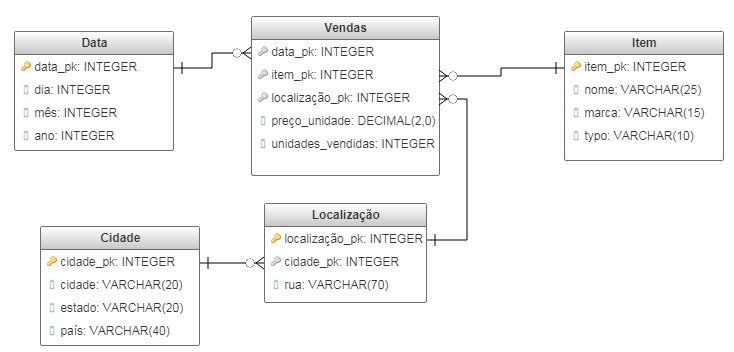
\includegraphics[width=13cm]{img/snow}
    \caption{Exemplo de esquema \textit{snowflake}}
    % \floatfoot{Adaptado da Figura \ref{fig:star_dim}}
	\label{fig:snow}
\end{figure*}

Para que possa ser construído um DW e aplicadas as modelagens acima descritas, 
é necessário alguma ferramenta que possa fazer o gerenciamento dele. 
De acordo com Elmasri e Navathe \cite{navathe2011banco} um banco de dados pode ser gerenciado por sistemas que 
facilitem este processo de gerenciamento no banco de dados. Antes de se ter um sistema que visava esse gerenciamento, entretanto, era utilizado para persistência de dados o sistema de arquivos. 

% SGBD ================================================================= %
\section{Sistemas Gerenciadores de Banco de Dados}

Apesar de simples, o sistema de arquivos apresentava alguns problemas por não oferecer suporte à redundância de informações; não garantir integridade de dados; 
falta de segurança; e o acesso e gerenciamento dos dados dependia de programas e aplicativos, fazendo com que seja necessário criar um novo aplicativo, ou adaptá-lo, a 
cada requisição de dados diferente. Outro problema crítico é não se ter informação de relacionamento entre arquivos diferentes.

Como forma de manter o gerenciamento de dados independente de aplicações e programas bem como solucionar os demais falhas do sistema de arquivos 
foram criados os Sistemas Gerenciadores de Banco de Dados, os SGBD. De acordo com Elmasri e Navathe \cite{navathe2011banco}, SGBD são uma coleção de programas para 
criação e manutenção de um banco de dados, que facilita a definição, construção, manipulação e compartilhamento de dados entre usuários e aplicações.

Dentre as vantagens que os SGBD trouxeram em detrimento ao sistema de arquivos estão:

\begin{itemize}
    \item{\textbf{Controle de redundância}}, para que não seja permitido duplicação de dados, pois isto causaria desperdício na capacidade de armazenamento.
    \item{\textbf{Restrição de acesso aos usuários}}, pois não será permitida manipulação do banco a todos os usuários, ou funcionários de uma empresa por exemplo.
    \item{\textbf{Execução de consultas eficiente}} através do uso de índices, normalmente implementadas utilizando hash ou árvores, para que o acesso ao disco seja mais rápido.
    \item{\textbf{Restrições de integridade}}, a fim de garantir que (i) dados não sejam inseridos de forma inconsistente de acordo com o tipo de atributo definido; 
    (ii) as relações entre entidades sejam efetuadas e (iii) restrições de chave sejam mantidas.
    \item{\textbf{Persistência de dados}}, para garantir que os dados serão inseridos e de fato armazenados no modelo.
    \item{\textbf{\textit{Backup}}} de dados periodicamente para evitar problemas caso aconteça alguma perda no banco e posterior \textbf{restauração}, para recuperar uma imagem do último backup feito no banco.
\end{itemize}

Existem várias classes de SGBD, conforme sua estruturação e a forma como manipulam os dados, 
entre as mais conhecidas estão o modelo relacional, objeto-relacional, orientado a 
objetos e a abordagem mais recente NoSQL.

\subsection{Modelo de SGBD Relacional}

O modelo mais utilizado de SGBD é o relacional, ou SGBDR (SGBD Relacional). Ele foi conceituado por 
Codd \cite{codd1970relational} em 1970 em um artigo no qual são expostas as 
vantagens de um modelo relacional em detrimento a um modelo de redes. 

Um modelo relacional define através de um conjunto de tabelas entidades que representam 
objetos do mundo real, cada qual com seus atributos. Esse conjunto de atributos é 
denominado registro do banco de dados, representando uma tupla, ou linha, na tabela. Assim como no mundo real, 
objetos devem estar também relacionados, e para tal SGBDR utilizam-se de chaves.

Em um SGBDR além de definir relacionamentos, as chaves também garantem integridade entre os dados. 
Existem dois tipos de chaves, uma que garante a unicidade de um atributo, ou seja, assegura que 
não haverão registros repetidos no banco tomando como referência aquele valor de chave, chamada de chave primária (do inglês \textit{Primary Key}, ou PK). A outra chave garante integridade no relacionamento entre duas entidades referenciando uma tabela na outra, que 
é a chave estrangeira (do inglês \textit{Foreign Key}, ou FK).

Tomando como exemplo uma empresa fictícia, são criados dois objetos reais que precisam ser 
representados sob a forma relacional, \textit{funcionário} e \textit{projeto}. Nesta empresa funcionários possuem \textit{nome, 
CPF, sexo, salário,} um \textit{supervisor} e trabalham em um ou mais \textit{projetos}. Esses projetos também possuem atributos: 
\textit{nome, código} e o número do \textit{departamento} no qual foram criados. Apenas com estas informações duas tabelas já são definidas 
no banco, \textit{funcionário} e \textit{projeto}, bem como seus atributos, como ilustra a Figura \ref{fig:func_proj}.

\begin{figure*}[htpb]
	\centering
		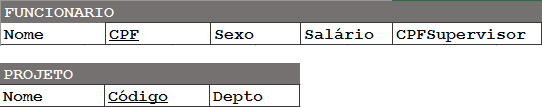
\includegraphics[width=13cm]{funcionario_projeto}
	\caption{Atributos das entidades \textit{funcionário} e \textit{projeto}}
	\label{fig:func_proj}
\end{figure*}

Como descrito, um funcionário trabalha em um ou mais projetos e ele precisa ainda registrar o número 
de horas trabalhadas nestes projetos. Desta forma é preciso de alguma forma relacionar funcionário com os projetos. 
Neste exemplo cabe a criação de uma nova entidade responsável unicamente por relacionar estes dois objetos e ainda 
armazenar o número de horas -- veja que o número de horas não cabe na tabela de funcionários nem na de projetos.

É nesta relação que são explorados os conceitos de chaves em um banco de dados. Para que a entidade que relaciona 
funcionário e projeto tenha informações de que funcionário trabalha em qual projeto é necessário acessar um número, ou código, 
definido para diferenciar todos os funcionários da empresa bem como o código do projeto e relacioná-los. Para o funcionário 
uma PK válida é o número do CPF e para o projeto o próprio atributo código. Essa relação pode ser nomeada unindo 
as entidades que relaciona, nesse caso \textit{funcionário\_projeto}, ou quando faz sentido pode ser nomeada de acordo com a função 
que realiza, neste caso como um funcionário trabalha em um projeto a relação pode ser \textit{trabalha\_em}.

O esquema que representa estas relações é como mostrado na Figura \ref{fig:relacao_func_proj}. Nela podemos ver as chaves primárias, em destaque, nas relações \textit{funcionário} e \textit{projeto}, e seus valores como chave estrangeira na relação \textit{trabalha\_em}. 

\begin{figure*}[htpb]
	\centering
		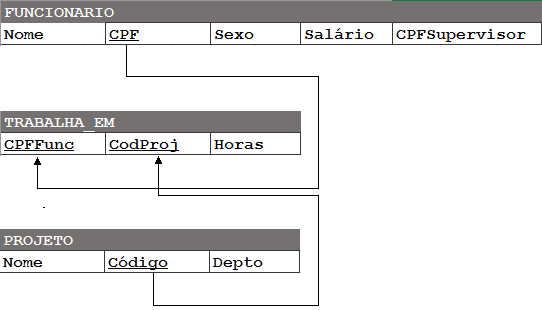
\includegraphics[width=13cm]{relacao_func_proj}
	\caption{Relacionamento entre \textit{funcionário} e \textit{projeto}}
	\label{fig:relacao_func_proj}
\end{figure*}

Modelos de bancos de dados prezam, sempre que possível, pela consistência de dados, principalmente se tomar operações transacionais como transações bancárias, que necessitam de um alto grau de consistência após operações de inserção e atualização, para que não haja perda de valores ou que esses ainda façam sentido no sistema. Por essa razão SGBDR seguem o conceito ACID (do inglês \textit{Atomicity, Consistency, Isolation, Durability}), o qual garante Atomicidade, Consistência, Isolamento e Durabilidade, ou Persistência, de dados. 

Modelos relacionais também seguem um alto grau de normalização nos dados a fim de evitar redundância e confusão entre atributos que podem ser desmembrados em outras entidades. Essa normalização é realizada normalmente até a Terceira Forma Normal, e o esquema final conterá um número maior de tabelas que o original devido ao desmembramento de atributos. Essa quantidade maior de tabelas acarreta no aumento de junções necessárias para recuperar atributos entre entidades relacionadas, ou seja, no aumento do acesso a entidades e no processamento de tuplas.

Além de diminuir o desempenho na recuperação de dados, um esquema normalizado causa um forte acoplamento entre tabelas, o que tornaria inviável o particionamento dos dados do banco em \textit{n} servidores como forma de escalar estes dados conforme seu volume aumenta, como é o caso de um ambiente analítico. Uma solução trivial para este problema é a denormalização de dados, porém para um SGBDR essa solução pode não ser viável, visto que sua implementação se dá seguindo a modelagem relacional.

Exemplos de SGBDR são PostgreSQL \cite{postgres2018r}, MySQL \cite{mysql2018r}, Microsoft SQL Server \cite{microsoft2018r}, SQLite \cite{lite2018r}, MariaDB \cite{maria2018r} e Oracle \cite{oracle2018r}. 

\subsection{Modelo de SGBD NoSQL}

% Bancos com o objetivo de suprir problemas apresentados por SGBDR começaram a emergir entre 2004 e 2007 visando alta escalabilidade, recuperação e armazenamento de grandes volumes de dados de forma eficiente, e ao mesmo tempo diminuir custos com hardware \cite{han2011nosql}. Esses bancos levaram o nome de NoSQL, porém isso não significa que não utilizam SQL para manipulação de dados.

% Detalhes sobre bancos de dados NoSQL são encontrados no Capítulo \ref{nosql}, no qual também é descrito o modelo colunar, utilizado por satisfazer os requerimentos de um ambiente de DW.

% \graphicspath{ {4-NoSQL/} }
% \chapter{Banco de Dados NoSQL}
% \label{nosql}

% NOSQL ==============================================================================================

O desenvolvimento de novas aplicações e surgimento de novas soluções 
para sistemas gerou crescimento no volume de dados de maneira acelerada. 
Com isso cresce também o número de usuários, necessitando portanto escalar 
o banco de dados. Existem duas soluções para escalar um sistema: o 
escalonamento vertical, que consiste em um \textit{upgrade} do servidor no 
qual o banco está hospedado; e o horizontal, aumentando o número de 
servidores e distribuindo o banco \cite{pritchett2008base, sharding2018educative}. 

Existem algumas desvantagens no \textit{upgrade} de um sistema. 
O banco de dados pode superar a capacidade da melhor configuração 
disponível no mercado, e ainda é caro por requerer a aquisição de 
uma configuração melhor. Mesmo considerado mais complexo, o 
escalonamento horizontal é mais viável. Entre as soluções apresentadas 
no particionamento horizontal em banco de dados estão o particionamento funcional e o 
\textit{sharding} \cite{pritchett2008base}. 

O particionamento funcional consiste em fragmentar os dados de acordo 
com a forma como são utilizados dado um contexto. Um esquema com quatro entidades, 
\textit{usuários}, \textit{produtos}, \textit{clientes} e \textit{endereço} 
pode ser distribuído em quatro servidores, 
um para cada entidade. Entidades que são utilizadas somente para leitura podem 
ser separadas de entidades onde dados são escritos, caracterizando outro 
exemplo de particionamento funcional. O problema com esta estratégia está 
no acoplamento entre entidades: se duas ou mais entidades estiverem 
relacionadas elas deverão estar no mesmo servidor, caso contrário não 
será possível atribuir as restrições de chave àquele relacionamento \cite{pritchett2008base}. 
Tomando o exemplo acima com as quatro entidades, supondo que \textit{cliente} 
e \textit{endereço} estejam relacionadas estas devem 
ser armazenados no mesmo servidor. 

A segunda estratégia, o \textit{sharding}, consiste em dividir os dados do banco 
utilizando algum critério de separação que não seja limitado à 
funcionalidade das entidades. Soluções como particionamento com base em 
\textit{hash} ou listas podem ser aplicadas. Considerando dez servidores e uma chave 
primária auto-incremental, a função de \textit{hash} pode tomar o módulo da chave 
primária pelo total de servidores como critério de seleção da partição 
na qual o dado será inserido. Utilizando uma lista é possível definir valores 
para os servidores e distribuir os dados de acordo com esses valores. 
Por exemplo, as linguagens C++, Java e C\# poderiam ser inseridas em uma 
partição destinada à linguagens orientadas a objeto.

O \textit{sharding} enfrenta problemas com junções entre dados, visto que os dados 
devem ser recuperados de diferentes partições e a maioria dos SGBDR não 
oferece suporte a chaves estrangeiras sob diferentes servidores, restando 
ao desenvolvedor tratar isso no código da aplicação \cite{pritchett2008base}. 
Uma solução para tais 
problemas é a denormalização de dados para que o número de junções diminua ou, 
no melhor dos casos e quando possível, seja zero. Contudo, isso é um problema 
para modelos relacionais, visto que trabalham sobre uma modelagem normalizada de dados. 
Além disso e de não se adaptarem à escalabilidade horizontal, 
são complexos e o fato de trazerem todas as informações de uma entidade sob a 
forma de tuplas causa lentidão em um ambiente analítico na recuperação de dados, 
cujas consultas percorrem o banco visando atributos específicos, processando 
somente o necessário. 

Outro problema crítico ao não utilizar a escalabilidade horizontal está na 
disponibilidade dos dados. Enquanto um banco se apoiar na escalabilidade vertical, 
qualquer queda no servidor acarretará na queda total no sistema de armazenamento, 
ao passo que quando se trabalha com servidores em paralelo a queda em uma máquina 
não trará prejuízos no conjunto todo. Assim, soluções como melhorar o hardware do 
servidor continuam sendo desvantajosas. 

Com o intuito de suprir tais problemas de escalabilidade, disponibilidade 
e recuperação rápida de dados, entre 2004 e 2007 os SGBD NoSQL começaram 
a ganhar destaque com o surgimento das bases de dados BigTable da Google \cite{chang2008bigtable}, e Dynamo 
da Amazon \cite{decandia2007dynamo}. O termo NoSQL, embora a princípio pareça indicar total independência 
de SQL, significa \textit{Not Only SQL}, “Não Apenas SQL”. Também, ele não descreve um 
único tipo de SGBD, mas sim uma classe de modelos, cada qual com suas propriedades. 
As mais conhecidas são quatro:

\begin{itemize}
    \item{\textbf{Orientado a Grafos}}, que se utiliza da Teoria dos Grafos para estruturar seus dados. 
    Um exemplo desta classe é o Neo4j \cite{neo2018nosql}.
    \item{\textbf{Orientado a Chave-Valor}}, que armazena os dados de forma similar a uma tabela \textit{hash}, 
    com uma chave referenciando um valor, ou tipo de dado. Exemplos são o Project Voldemort \cite{voldemort2018nosql}, 
    DyanmoDB \cite{amazon2018nosql}, o Riak \cite{riak2018nosql} e o Redis \cite{redis2018nosql}.
    \item{\textbf{Orientado a Documento}}, uma versão melhorada do Chave-Valor, 
    no qual os valores são armazenados como documentos através de estruturas complexas como JSON e XML. 
    Exemplos são o MongoDB \cite{mongo2018nosql} e o CouchDB \cite{couch2018nosql}.
    \item{\textbf{Orientado a Colunas}}, ou modelo colunar, 
    que utiliza tabelas como armazenamento de entidades, 
    porém não agrupa os dados sob forma de tuplas, e sim colunas. Exemplos são o MonetDB \cite{monetdb2017c}, C-Store \cite{cstore2018nosql}, BigTable \cite{google2018nosql} e Cassandra \cite{cassandra2018nosql}.
\end{itemize}

De maneira geral, as vantagens no uso de um SGBD NoSQL estão no rápido processamento de um grande volume de dados, flexibilidade para expansão e baixo custo de escalabilidade. Devido ao vasto número de SGBD dentro de cada classe de NoSQL, esses banco de dados também podem ser classificados de acordo com o Teorema CAP (do inglês \textit{Consistency, Availability, Partition tolerance}). Segundo Eric Brewer \cite{brewer2000towards, gilbert2002brewer}, um sistema distribuído não é 
capaz de conciliar consistência, disponibilidade e tolerância a partição de dados simultaneamente, tendo que optar por apenas dois destes. 
SGBDR prezam por disponibilidade e consistência de dados seguindo ACID, porém, a preocupação com consistência 
pode tornar a manipulação de dados lenta. Visto que o movimento NoSQL surgiu com a intenção de 
melhorar a escalabilidade e disponibilidade de dados, e tornar a manipulação destes mais rápida, 
a maioria deles trabalha com os atributos de disponibilidade e tolerância à partição. 
Essa configuração assume um conceito diferente do ACID para bancos NoSQL, e Pritchett \cite{pritchett2008base} propôs um teorema diferente deste, mais otimista, onde a consistência é relaxada, o Teorema BASE (\textit{Basically Available, Soft State, Eventual Consistency}).

O Teorema BASE assume que a consistência em um banco 
de dados está em estado de fluxo, ao contrário de ACID que força a consistência a cada operação, 
sendo este considerado por Pritchett \cite{pritchett2008base} um método pessimista. 
Neste cenário a disponibilidade é garantida devido à tolerância a partição, fazendo 
com que a falha de um servidor não cesse o funcionamento de todo o sistema -- por exemplo, caso uma partição falhe em um sistema rodando sobre dez servidores, apenas 10\% dos dados estarão indisponíveis e somente os usuários daquela partição serão afetados.

% COLUNAR =============================================================================

% \subsubsection{Modelo de SGBD NoSQL Colunar}

Dentre as categorias de bancos de dados NoSQL citadas a que melhor se adequa aos 
propósitos analíticos é a colunar. Sistemas colunares armazenam seus dados 
em colunas que representam atributos das entidades, fazendo com que apenas os atributos necessários sejam 
lidos \cite{khoshafian1987query}, o que diminui o tempo de acesso 
ao disco \cite{matei2010column, abadi2008column}. Cada uma destas colunas pode armazenar seus valores utilizando o par 
\textit{chave, valor} \cite{abadi2013design, khoshafian1987query}, sendo esta uma das formas de implementação 
de um sistema colunar. 
A Figura \ref{fig:row-col} ilustra de forma simples, embora apenas visual, 
a diferença principal entre um armazenamento utilizando linhas, conforme a Figura \ref{fig:row}, e outro utilizando 
colunas, Figura \ref{fig:column}, a partir dos registros da Figura \ref{fig:regs}, baseada na entidade \textit{funcionário} apresentada no Capítulo \ref{sgbd}.

% (descrita na Seção \ref{sec:implementacao_col} deste capítulo)

\begin{figure*}[htpb]
	\centering
		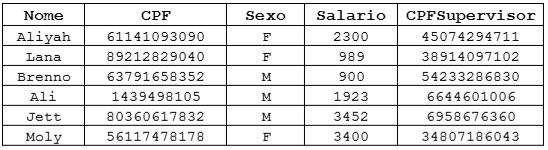
\includegraphics[width=12cm]{registros}
	\caption{Exemplos de registros para a entidade \textit{funcionário} apresentada no Capítulo \ref{sgbd}}
	\label{fig:regs}
\end{figure*}

\begin{figure*}[htpb]
    \centering
    \subfigure[]{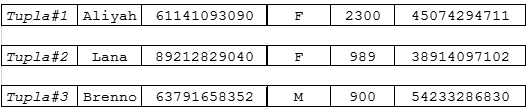
\includegraphics[width=8cm]{row}\label{fig:row}}
    \subfigure[]{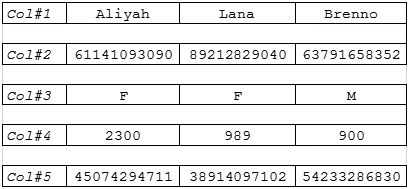
\includegraphics[width=6.8cm]{column}\label{fig:column}}
    \caption{Diferença visual entre registros armazenados em um banco relacional e colunar}
    \label{fig:row-col}
\end{figure*}

Matei \cite{matei2010column} cita algumas vantagens de sistemas colunares:

\begin{itemize}

    \item{\textbf{Melhor desempenho}}, pela forma com que os dados são armazenados e o uso de índices 
    visando o armazenamento ao invés de localização de registros, resultando em menos operações de 
    entrada e saída.
    \item{\textbf{Rápidas operações de agrupamento}}, bastante utilizadas em ambientes OLAP, visto 
    que valores de um mesmo atributo são armazenados consecutivamente. Bem como operações matemáticas, 
    como recuperar o maior ou menor valor, soma e média.
    \item{\textbf{Alta compressão de dados}} pode ser alcançada, devido às chances de se ter 
    valores repetidos para um mesmo atributo serem maiores.

\end{itemize}

Existem diferentes abordagens para se implementar um SGBD colunar. Essas abordagens levam em conta 
mudanças na codificação de um banco, apenas na modelagem dele, bem como se será possível atingir 
níveis altos de compressão. A primeira técnica consiste no \textbf{particionamento vertical} dos dados, a 
segunda em \textbf{modificar a camada de armazenamento} e a terceira corresponde a junção de ambas.

% \subsection{Implementação do Sistema Colunar}
% \label{sec:implementacao_col}

Antes de detalhar os métodos de implementação de um banco de dados colunar, é fundamental discutir sobre a reconstrução de tuplas nesse tipo de SGBD. 
Segundo Abadi et al. \cite{abadi2007materialization}, a parte lógica e visual de um banco de dados colunar se apresenta da mesma forma que 
um relacional. Isso faz com que a maioria dos SGBD colunares ofereçam uma interface relacional de comunicação, compatível com os padrões.

Como os atributos de um modelo colunar acabam ficando separados em disco um do outro, eles precisam ser unidos novamente em tuplas para 
que o resultado de uma consulta seja exibido. Existem duas técnicas para realizar essa reconstrução, ou materialização: \textit{Early Materialization} (EM) e 
\textit{Late Materialization} (LM) \cite{abadi2007materialization, abadi2008query}.

A técnica de \textit{Early Materialization}, melhor traduzida como materialização prévia nesse contexto, é a política adotada por banco de dados relacionais, e consiste 
em adicionar as colunas à tupla conforme a coluna é requisitada na consulta. Essa técnica não leva em conta o predicado da consulta. Como exemplo, considere a consulta a seguir:

\begin{lstlisting}[language=SQL,label=sql_1]
                    SELECT nome FROM funcionario 
                    WHERE salario >= 1000 AND sexo='F'
\end{lstlisting}

A EM irá processar essa consulta e construir uma tupla com os atributos \textit{nome, salário} e \textit{sexo}, com todos os registros 
armazenados em banco. Considere que os registros são como mostrados na Figura \ref{fig:regs}, o construtor de tuplas retornará os registros conforme a Figura \ref{fig:em}. Esse método só analisa o predicado após a construção das tuplas, o que não acontece na LM. 

\begin{figure*}[htpb]
	\centering
        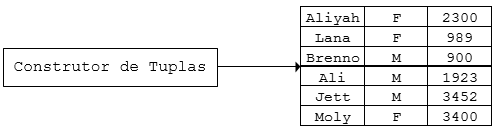
\includegraphics[width=14cm]{em}
	\caption{Tuplas reconstruídas a partir da \textit{Early Materialization}}
	\label{fig:em}
\end{figure*}

Na LM, ou materialização tardia, é analisado primeiro o predicado e verificado quais valores atendem a esse predicado em cada coluna. 
No caso da SQL acima primeiro seria analisado o predicado de seleção, nesse caso \texttt{WHERE salario >= 1000 AND sexo='F'}, e então 
através do operador lógico AND seria possível retornar a posição dos atributos que satisfazem essa seleção, para então 
construir a tupla a partir do predicado de projeção somente com o atributo \textit{nome}. Em suma, apenas após ter a posição de cada atributo é que a tupla é construída, descartando a reconstrução de tuplas que seriam posteriormente descartadas. A Figura \ref{fig:lm} apresenta o resultado após a construção das tuplas na LM.

\begin{figure*}[htpb]
	\centering
        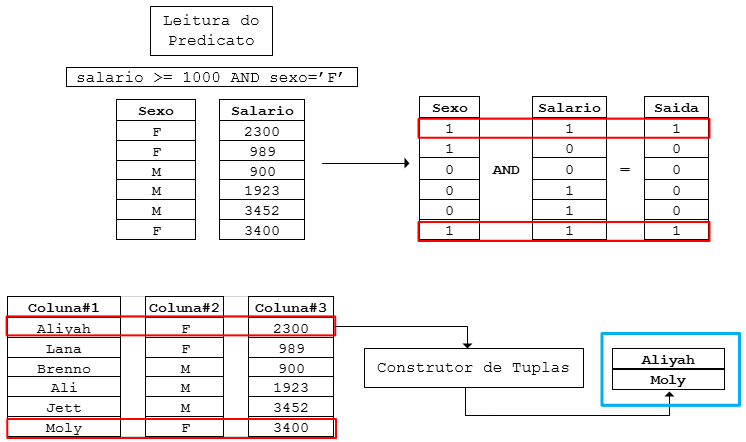
\includegraphics[width=14cm]{lm}
	\caption{Tuplas reconstruídas a partir da \textit{Late Materialization}}
	\label{fig:lm}
\end{figure*}

% inserir subfigure com tuplas

% \subsection{Particionamento Vertical}

A primeira técnica de implementação de um banco de dados colunar consiste no particionamento vertical dos dados. Considerada a técnica mais simples para implementar um banco colunar, esta técnica 
realiza a partição dos dados de forma que cada atributo de uma entidade seja armazenado 
em uma tabela de duas colunas contendo o par <chave/índice, valor do atributo> \cite{khoshafian1987query}.

% inserir figura de particionamento vertical

A Figura \ref{fig:vertical} mostra que é possível desmembrar o esquema relacional da Figura \ref{fig:regs} em colunas de atributos -- foram desmembrados os atributos \textit{nome, sexo} e \textit{salario}. 
No momento em que uma consulta analítica é realizada, não serão processados dados além 
dos de fato requeridos e nenhum dado é perdido pois ainda haverá referência entre os atributos 
através das chaves.

\begin{figure*}[htpb]
	\centering
        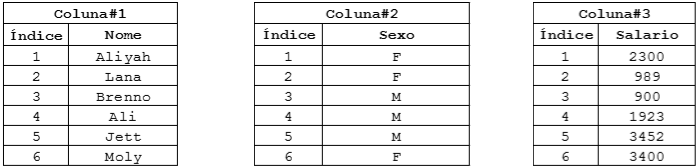
\includegraphics[width=\textwidth]{vertical}
	\caption{Implementação do modelo colunar utilizando particionamento vertical}
	\label{fig:vertical}
\end{figure*}

Essa abordagem é a mais simples de se implementar, pois nenhuma mudança é feita 
na codificação do banco de dados, sendo que a única alteração necessária está a nível 
da aplicação responsável por executar as consultas, mudando a lógica de acesso aos dados. Isso torna prático para empresas a 
mudança entre a estratégia relacional e a colunar, pois torna possível o uso de um mesmo 
SGBD como DW.

Ao mesmo tempo que essa implementação traz praticidade na migração de dados, ela não difere 
muito da abordagem relacional no que concerne ao desempenho. Em Abadi \cite{abadi2008query} 
é mostrado que adaptar dados de um esquema relacional utilizando particionamento vertical não 
trouxe melhoras no desempenho das consultas. Foi verificado que o custo de junções para unir 
as colunas é alto conforme a quantidade de atributos selecionados aumenta e não foi possível 
usufruir eficientemente da compressão de dados.

% \subsection{Modificação na Camada de Armazenamento}

A segunda abordagem para implementar um sistema colunar consiste em já modificar o armazenamento do banco. Essa técnica não altera a parte 
lógica da modelagem do banco, mas a camada física alterando o armazenamento de 
linha por linha para coluna por coluna. Nessa implementação as chaves não precisam ser 
repetidas como na abordagem anterior, na qual a primeira coluna de cada tabela 
consistia no valor de chave da cada atributo. O \textit{i-ésimo} valor de atributo 
de uma coluna estará associado ao \textit{i-ésimo} atributo das demais colunas e 
não é desperdiçado espaço em disco com as chaves.

Neste método a reconstrução de tuplas é realizada antes da execução da consulta de fato. Como apenas um determinado número de atributos precisa ser acessado, estes são combinados seguindo a lógica que o \textit{i-ésimo} atributo de uma coluna está relacionado com o \textit{i-ésimo} atributo das demais. Aqui tem-se uma vantagem no modelo orientado a linhas, por este já armazenar as sob o formato de linhas e não precisar armazenar os dados em ordem.

% \subsection{Modificação na Camada de Armazenamento e Particionamento Vertical}

A última, e melhor, abordagem consiste em modificar a camada de armazenamento do banco de dados e a aplicação que processa as consultas \cite{stonebraker2005c, boncz2005monetdb}, assim o processador pode manter os dados sob a forma de colunas sem precisar unir as colunas e construir tuplas. Uma vantagem óbvia desta técnica é a eliminação da reconstrução de tuplas e com isso menos dados precisam ser previamente movimentados, diminuindo 
o tempo de processamento.  

% \section{Compressão de Dados}

Além da diferença na implementação, e por consequência disso, uma característica marcante de um SGBDC é a alta possibilidade de compressão de dados. 
Existem diversas formas de comprimir os dados, porém deve-se ater ao fato de 
que o tempo de compressão e descompressão não deve afetar significativamente o processamento 
dos dados no SGBD. Para tal, uma solução é utilizar métodos que consigam operar sob os dados 
ainda comprimidos -- ainda nesta seção são apresentados alguns dos algoritmos utilizados para 
compressão em banco de dados.

Como exemplo, apenas ilustrativo, de como os dados em um sistema colunar podem ser comprimidos de forma mais 
eficiente que em um relacional, considere a entidade \textit{usuário} a seguir, com os 
atributos \textit{id, nome, idade} e \textit{sexo}. A primeira coluna corresponde aos índices utilizados no banco. 

\begin{verbatim}
    1: 0, Bruno, 50, M
    2: 10, João, 23, M
    3: 20, Maria, 30, F
    4: 90, Ana, 23, F
    5: 78, Gabriel, 23, M
\end{verbatim}

Um banco relacional armazena estes atributos da forma como foram apresentados acima. 
Considerando o armazenamento colunar, os mesmos dados seriam armazenados da seguinte forma: 

\begin{verbatim}
    1: 0, 2: 10, 3: 20, 4: 90, 5: 78
    1: Bruno, 2: João, 3: Maria, 4: Ana, 5: Gabriel
    1: 50, 2: 23, 3: 30, 4: 23, 5: 23
    1: M, 2: M, 3: F, 4: F, 5: M
\end{verbatim}

Note que fica mais claro que como os atributos são armazenados em uma coluna com chave e valor 
existirão mais chances de repetição de valores em uma mesma coluna. Os atributos \textit{idade} e 
\textit{sexo} se repetem para alguns registros, possibilitando assim compressão destes dados. 
Comprimindo estas repetições o nosso modelo é armazenado da forma: 

\begin{verbatim}
    1: 0, 2: 10, 3: 20, 4: 90, 5: 78
    1: Bruno, 2: João, 3: Maria, 4: Ana, 5: Gabriel
    1: 50, 2, 4, 5: 23, 3: 30
    1, 2, 5: M, 3, 4: F
\end{verbatim}

Westmann \textit{et al.} \cite{westmann2000implementation} consideram que os métodos de compressão em um banco de dados devem ser capazes de se aplicar 
no banco como um todo, bem como em uma tupla ou a cada atributo de tupla, e serem rápidos em processamento quando há casos em que seja 
necessário realizar descompressão.

O primeiro método consiste em comprimir a representação de valores inteiros, baseado no algoritmo \textit{null supression} \cite{westmann2000implementation, roth1993database}. A ideia é descartar zeros na representação de um inteiro de quatro bytes, por exemplo, 
ao invés de se representar o número 10 da forma '00000000000000000000000000001010', seriam utilizados apenas quatro bits, '1010'. É 
necessário entretanto, guardar a informação de quantos bits são utilizados para armazenar um número e em alguns casos também é preciso 
armazenar um bit a mais para o sinal do inteiro. Esse algoritmo pode ser utilizado para comprimir o tamanho de strings no banco 
quando estas são representadas pelo tipo VARCHAR, visto que para esse tipo de dado o tamanho também é armazenado devido a possibilidade 
deste variar.

Um método bastante empregado é a Codificação por Dicionário. Nele atributos que possuem um padrão fixo, por exemplo, os números primos de 
3 a 19 (3, 5, 7, 11, 13, 17, 19), podem ser representados por um dicionário de 3 bits. Este algoritmo pode ser utilizado para compressão 
de valores NULL, considerando-o como um possível valor no padrão.

Abadi, Madden e Ferreira \cite{abadi2006integrating} utilizam a compressão por dicionário e uma variação do algoritmo \textit{null supression} para implementar o banco de dados C-Store e ainda apresentam dois outros métodos. O primeiro é o \textit{run-length}, que pode ser bem aproveitado 
em bancos colunares quando atributos são repetidos sequencialmente e possuem pouca variação. Ele consiste em contar o número de vezes no qual 
um valor é repetido utilizando a tripla (valor, posição inicial, tamanho). 
% Um exemplo é ilustrado na Figura A com o atributo \textit{especialização}.



% inserir uma imagem run length com graduação, mestrado, doutorado.

O último método apresentado pelos autores é a Codificação por Vetor de Bit, bastante útil quando uma coluna possui número limitado 
de possibilidades, como linguagens de programação dentro de um dado paradigma ou estados do Brasil. Uma string de bits representa a 
ocorrência do valor de atributo, onde '1' representa a ocorrência naquela posição e '0' a não ocorrência. Como exemplo, uma coluna com os 
valores {M M F M F F M} podem ser representados pela cadeia de bits 1 1 0 1 0 0 1 para o valor M, e 0 0 1 0 1 1 0 para F.

Em suma, ao implementar um banco colunar tanto a aplicação deve ser capaz de entender e conseguir recuperar informações mesmo comprimidas, como a modificação da camada de armazenamento deve ser implementada tal que se possa usufruir de algum método de compressão. Caso contrário um 
dos principais diferenciais de modelos colunares não será explorado e poderá não haver impacto no desempenho quando trabalhado com uma 
grande massa de dados, como é a realidade de empresas.

\section{Considerações Finais}

% data warehouses e olap -> modelo denormalizado -> sgbdr x sgbdc

Tendo surgido como solução para dar suporte à tomada de decisão, DWs precisam ter seus dados recuperados de forma eficiente. A principal discussão acerca disso está em torno de qual modelagem utilizar e como realizar o gerenciamento deste repositório de forma a conseguir um bom desempenho na recuperação de dados como informação útil à uma empresa. Como solução a isso estão os SGBDR, entretanto, seu uso causa queda no desempenho conforme o volume de dados aumenta, para tanto são necessários outros meios de gerenciamento que possam lidar com esse grande volume de dados.

Apresentando soluções aos impasses de um SGBDR estão os SGBD NoSQL, e dentre suas classes a que melhor supre as necessidades de um ambiente analítico é a colunar. Com uma implementação diferente da utilizada pelos SGBDR, este SGBD possibilita altas taxas de compressão e recuperação de atributos específicos sem processar mais do que o requisitado por uma consulta. 

Empresas ainda utilizam SGBDR para gerenciar DWs, e para analisar qual SGBD é melhor nesta função pode-se aplicar alguma métrica para cálculo de desempenho e comparar um com o outro, ou vários. Esse cálculo deve considerar ainda as possíveis modelagens entre os SGBD, possibilitando adaptar diferentes modelagens dentro de um DW. Na área de banco de dados são utilizados \textit{benchmarks} produzidos por empresas com foco em desenvolver padrões no processo de transações.